%! Author = Son Trinh
%! Date = 10/13/2022

\begin{frame}{Gaussian Processes (GP) -- method summary}

\maketag{regression} \maketag{classification} \maketag{nonparametric} \maketag{probabilistic}

\medskip

\highlight{General idea}
\begin{itemize}
  \item GP approach determines a distribution across the potential functions $\bm{f}$ that suit the observed data.
  \item It is based on the "prior" assumption that neighboring observations should be correlated with each other.
  \item It assumes that the observations are normally distributed, and that the coupling between them occurs through the use of a normal distribution's covariance matrix.
  \item \textbf{Predict} via the maximum a-posteriori (MAP) estimate.
\end{itemize}

\medskip

\highlight{Hypothesis space} ~~
$\Hspace = \left\{ \bm{f} = \left[f\left(\xi[1]\right), \dots, f\left(\xi[n]\right)\right] \sim \mathcal{N}\left(\bm{m}, \bm{K}\right) ~|~ \bm{m} \in \R^n, \bm{K} \in \R^{n\times n} \right\}$

\medskip

\begin{minipage}[b]{0.5\textwidth}
  % FIGURE SOURCE: https://docs.google.com/presentation/d/1xodP6ayu1Gay6mMKgzVWYEFmSoeG5kNuqsaTkFFmd78  /edit
  \centering
  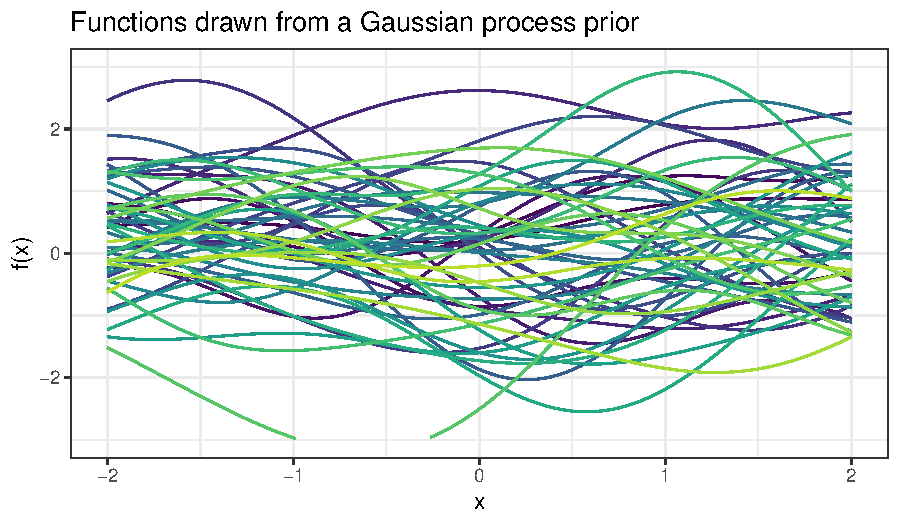
\includegraphics[width=0.9\textwidth]{figure/gp-prior} \\
\end{minipage}%
\begin{minipage}[b]{0.5\textwidth}
\centering
  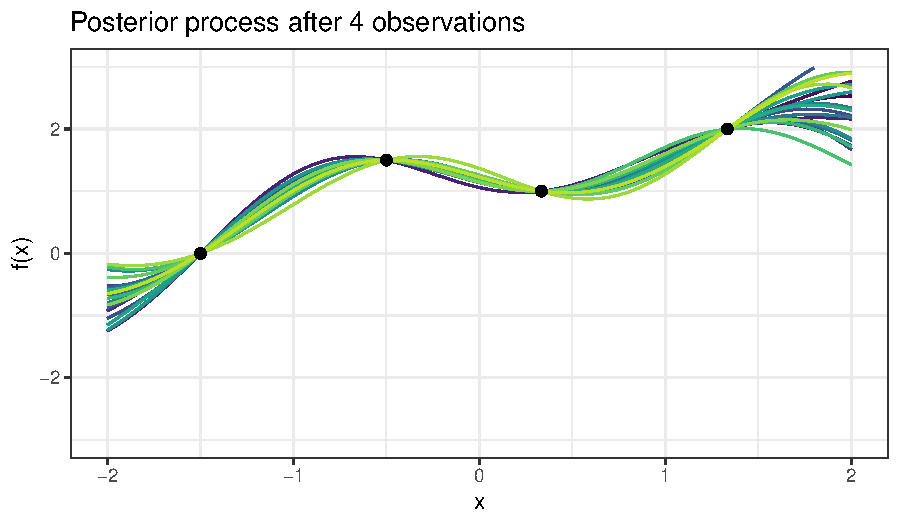
\includegraphics[width=0.9\textwidth]{figure/gp-posterior}
\end{minipage}

\end{frame}

% ------------------------------------------------------------------------------

\begin{frame}{Gaussian Processes (GP) -- Pro's \& Con's}

\begin{columns}[onlytextwidth]
  \begin{column}{0.5\textwidth}
    \highlight{Advantages}
    \footnotesize
    \begin{itemize}
      \positem GP allows to \textbf{quantify prediction uncertainty} induced by both intrinsic noise in the problem and errors in the parameter estimation process.
      \positem GP is a function \textbf{interpolator}. It can "predict" the exact value of a training point.
      \positem GP is \textbf{non-parametric} and can model virtually any functions of observations.
    \end{itemize}
  \end{column}
  \begin{column}{0.5\textwidth}
    \highlight{Disadvantages}
    \footnotesize
    \begin{itemize}
      \negitem GP is \textbf{not sparse}, i.e., it uses the whole training set for prediction.
      \negitem GP is \textbf{not particularly easy to understand} conceptually at first sight.
    \end{itemize}
  \end{column}
\end{columns}

\vfill

\small

\conclbox{Powerful predictor with built-in measurement for uncertainty, suitable for small data sets}

\end{frame}

% ------------------------------------------------------------------------------

\begin{frame}{Gaussian Processes (GP) -- Practical hints}

\highlight{Sparse Gaussian Processes}
\begin{itemize}
	\item The sparse version of the original Gaussian Processes
	\item Suitable for large sample size
\end{itemize}

\medskip

\highlight{Implementation}

\begin{itemize}
  \item \textbf{R:} \texttt{mlr3} learners \texttt{LearnerClassifGausspr} /
    \texttt{LearnerRegrGausspr}, calling \texttt{kernlab::gausspr()}
  \item \textbf{Python:} \texttt{GaussianProcessClassifier} /
  \texttt{GaussianProcessRegressor} from package \texttt{scikit-learn}
\end{itemize}

\end{frame}